\documentclass[]{article}
\usepackage{graphicx}
\graphicspath{ {./images/} }

%opening
\title{CSCI 470 - Note-taking application requirements}
\author{Logan Humbert}

\begin{document}
	
	\maketitle
	
	\pagebreak
	
	\section{Description of the application}
	
	This little mobile application aims to let students taking notes for their different classes, and organizing them by class.
	
	\section{Requirements}
	
	\begin{itemize}
		\item \textbf{Who are the users? } The users are students (College, High School, Middle School, ...)
		
		\item \textbf{Who are the customers?} This app is only made in a school context. There is no real customer for it.
		
		\item  \textbf{User stories:}
			\begin{itemize}
				\item As a new user, I want to add my different classes, and start adding notes for them
				
				\item  As a regular user, I keep adding a new note during a lecture in my different classes, then I review them when I study.
				I can easily modify the content of the note if I need to.
			\end{itemize}
		
	\end{itemize}
	
	\section{Features}
	
	The user should be able to complete these different tasks easily:
	
	\begin{itemize}
		\item See his different classes
		\item Add/edit or delete a class
		\item Create/edit/delete a note for any class he has created
		\item View a note
		\item  Search for a class or a note by typing a part of its name
	\end{itemize}
	
	\pagebreak
	
	\section{Design}
	
	Here is a first sketch of the different pages of the app, and the transitions between them:
	
	\begin{figure}[!htb]
		\centering
		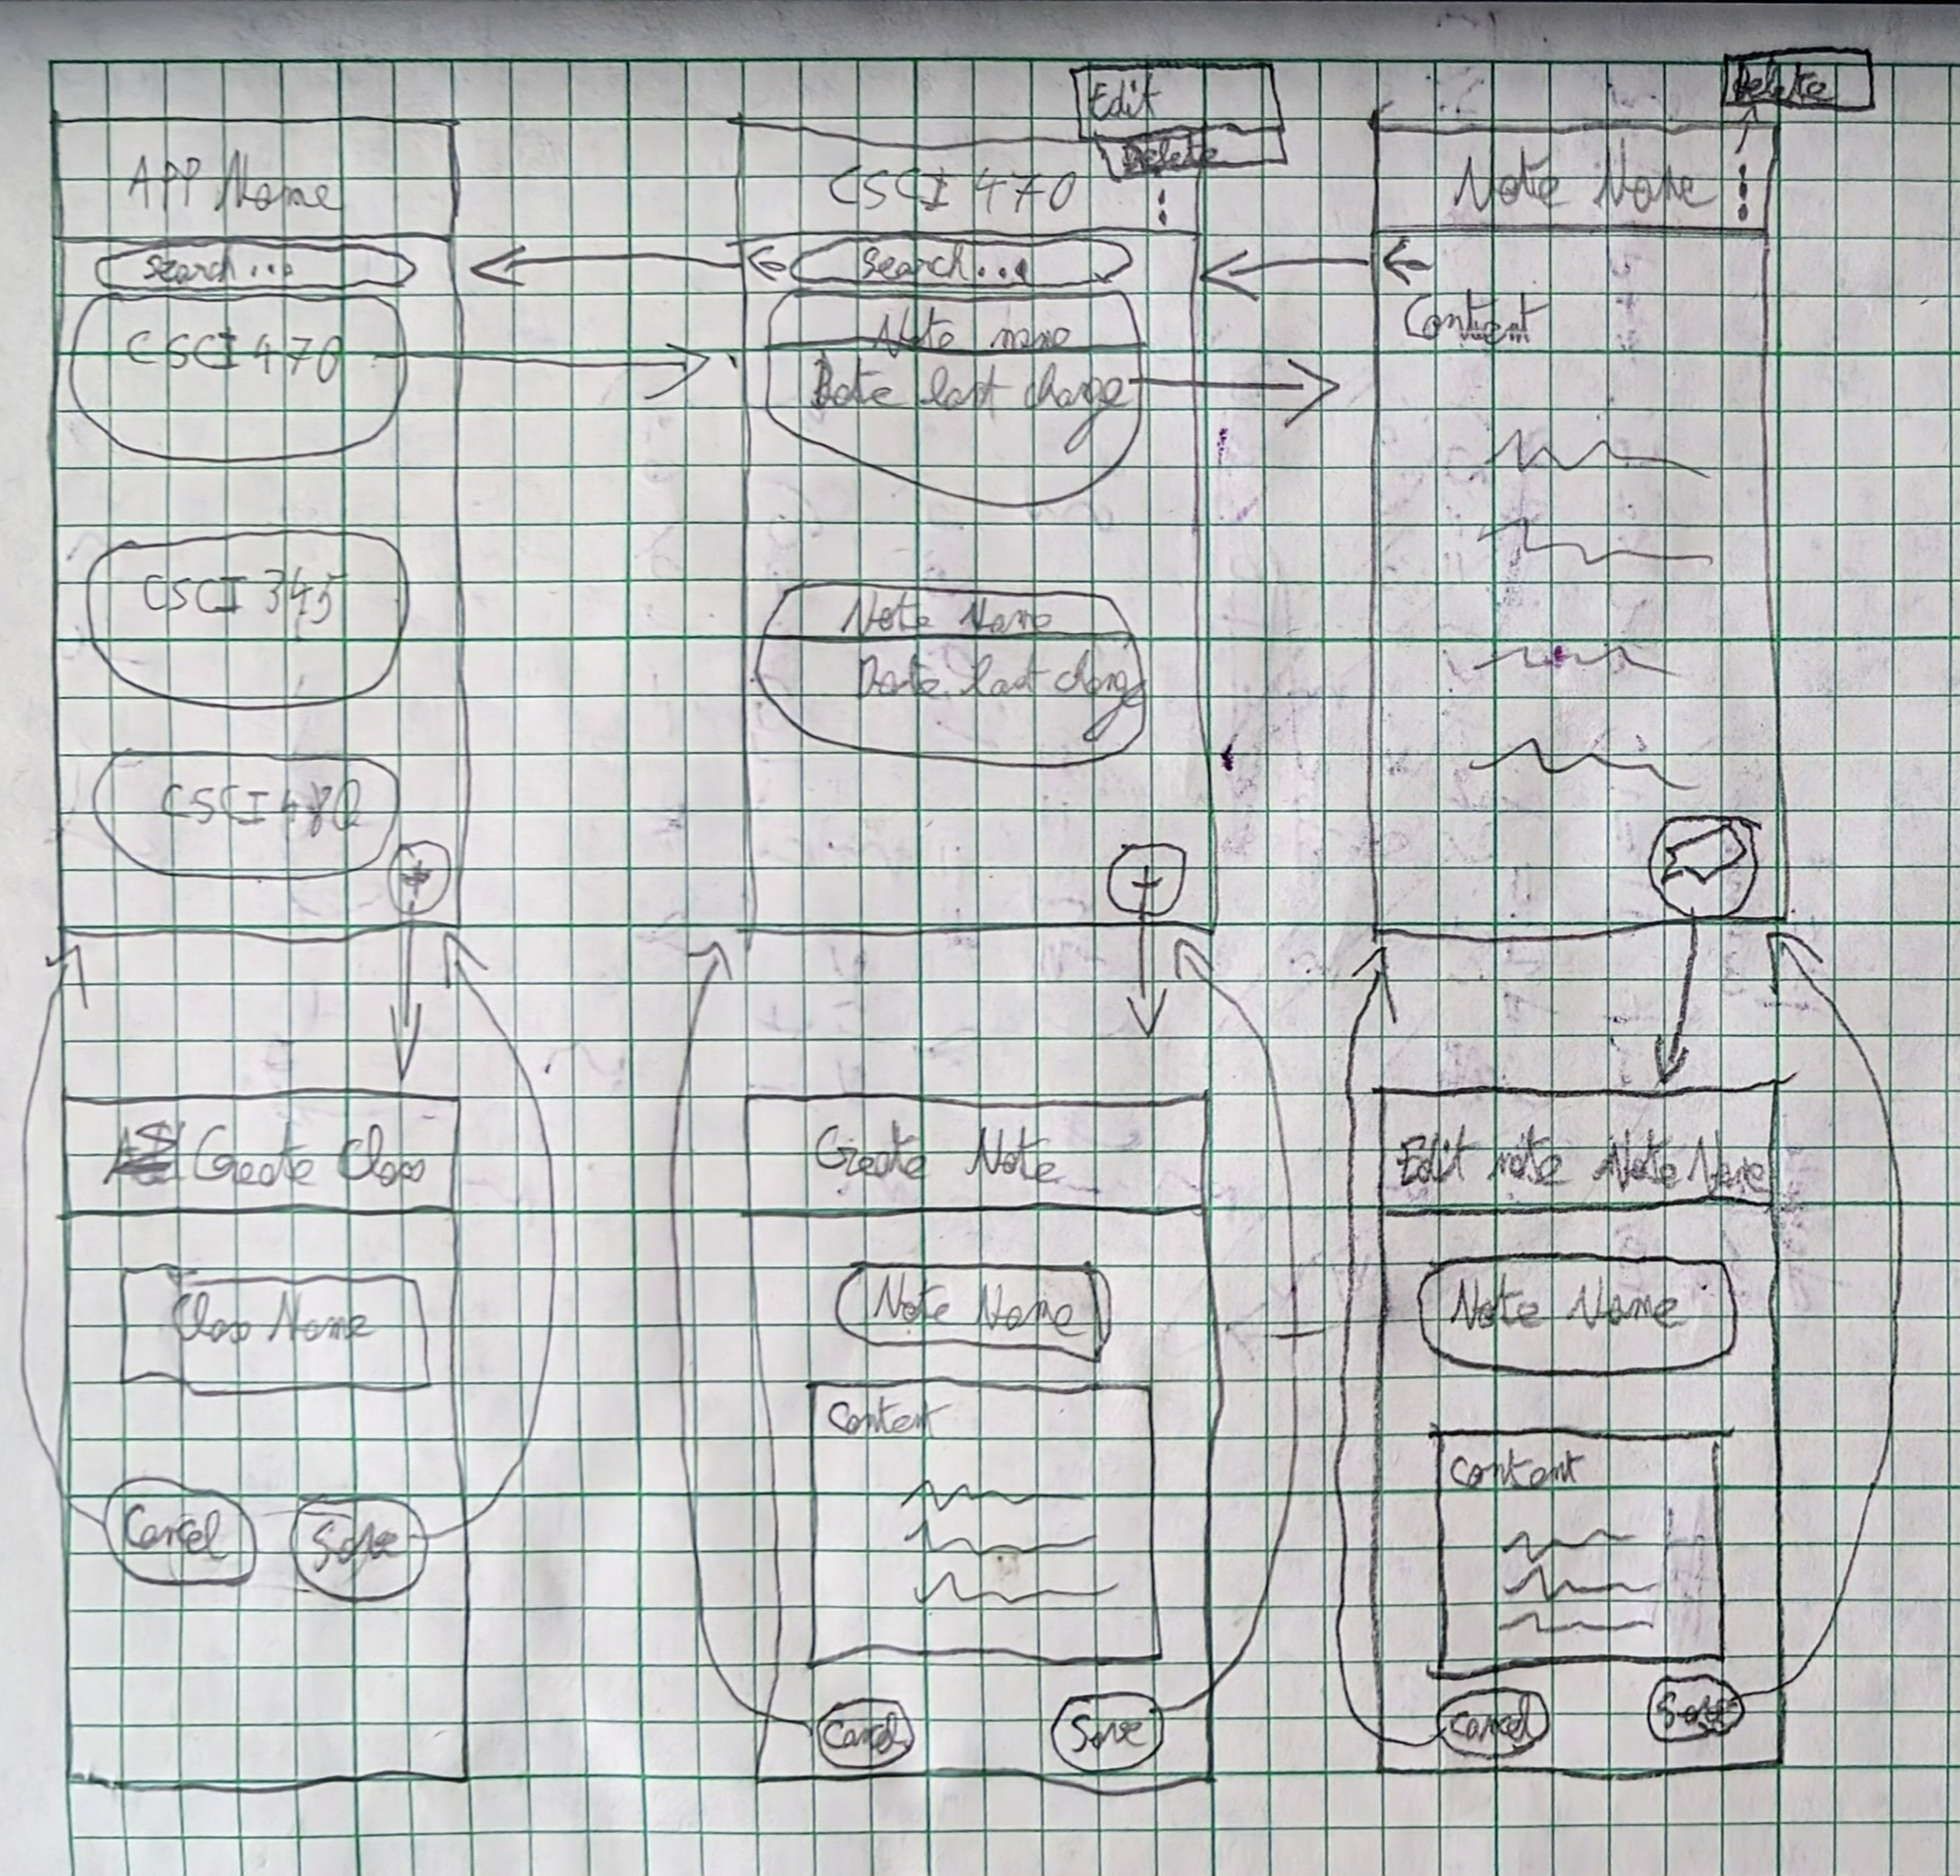
\includegraphics[scale=0.1]{first_sketch}
		\caption{First sketch on paper}
	\end{figure}
	
	I imagine having 5 different screens:
	
	\begin{itemize}
		\item The home page, containing a list of the existing classes.
		\item The add/edit class form
		\item The list of notes in a class
		\item The add/edit note form
		\item The content of a note
	\end{itemize}
	
	All pages can be accessed by clicking on a specific element, as the arrows on the sketches show.
	
\end{document}